\documentclass{standalone}

\usepackage{tikz}

\def \D { 0/0 , 5/0 , 10/0 , 15/0 , 20/0 , 4/2 , 1/3 , 11/3 , 16/3 , 21/3 , 3/4 , 15/5 , 20/5 , 2/6 , 12/6 , 1/8 , 6/8 , 16/8 , 21/8 , 3/9 , 13/9 , 0/10 , 5/10 , 20/10 ,  7/11 , 12/11 , 17/11 , 4/12 , 19/12 , 24/12 , 11/13 , 21/13 , 3/14 , 8/14 , 18/14 , 23/14 , 12/16 , 22/16 , 4/17 , 9/17 , 21/18 , 3/19 , 8/19 , 13/19 , 23/19 , 20/20 , 4/22 , 9/22 , 14/22 , 19/22 , 24/22 }

\def \A { 0/0 , 10/0 , 15/0 , 20/0 , 1/3 , 11/3 , 15/5 , 20/5 , 2/6 , 12/6 , 6/8 , 16/8 , 3/9 , 20/10 ,  7/11 , 17/11 , 11/13 , 21/13 , 3/14 , 8/14 , 12/16 , 22/16 , 3/19 , 8/19 , 13/19 , 23/19 }

\def \B {5/0 , 4/2 , 16/3 , 21/3 , 3/4 , 2/6 , 1/8 , 6/8 , 21/8 , 13/9 , 5/10 , 20/10 , 12/11 , 4/12 , 19/12 , 24/12 , 23/14 , 22/16 , 4/17 , 9/17 , 21/18 , 20/20}

\begin{document}
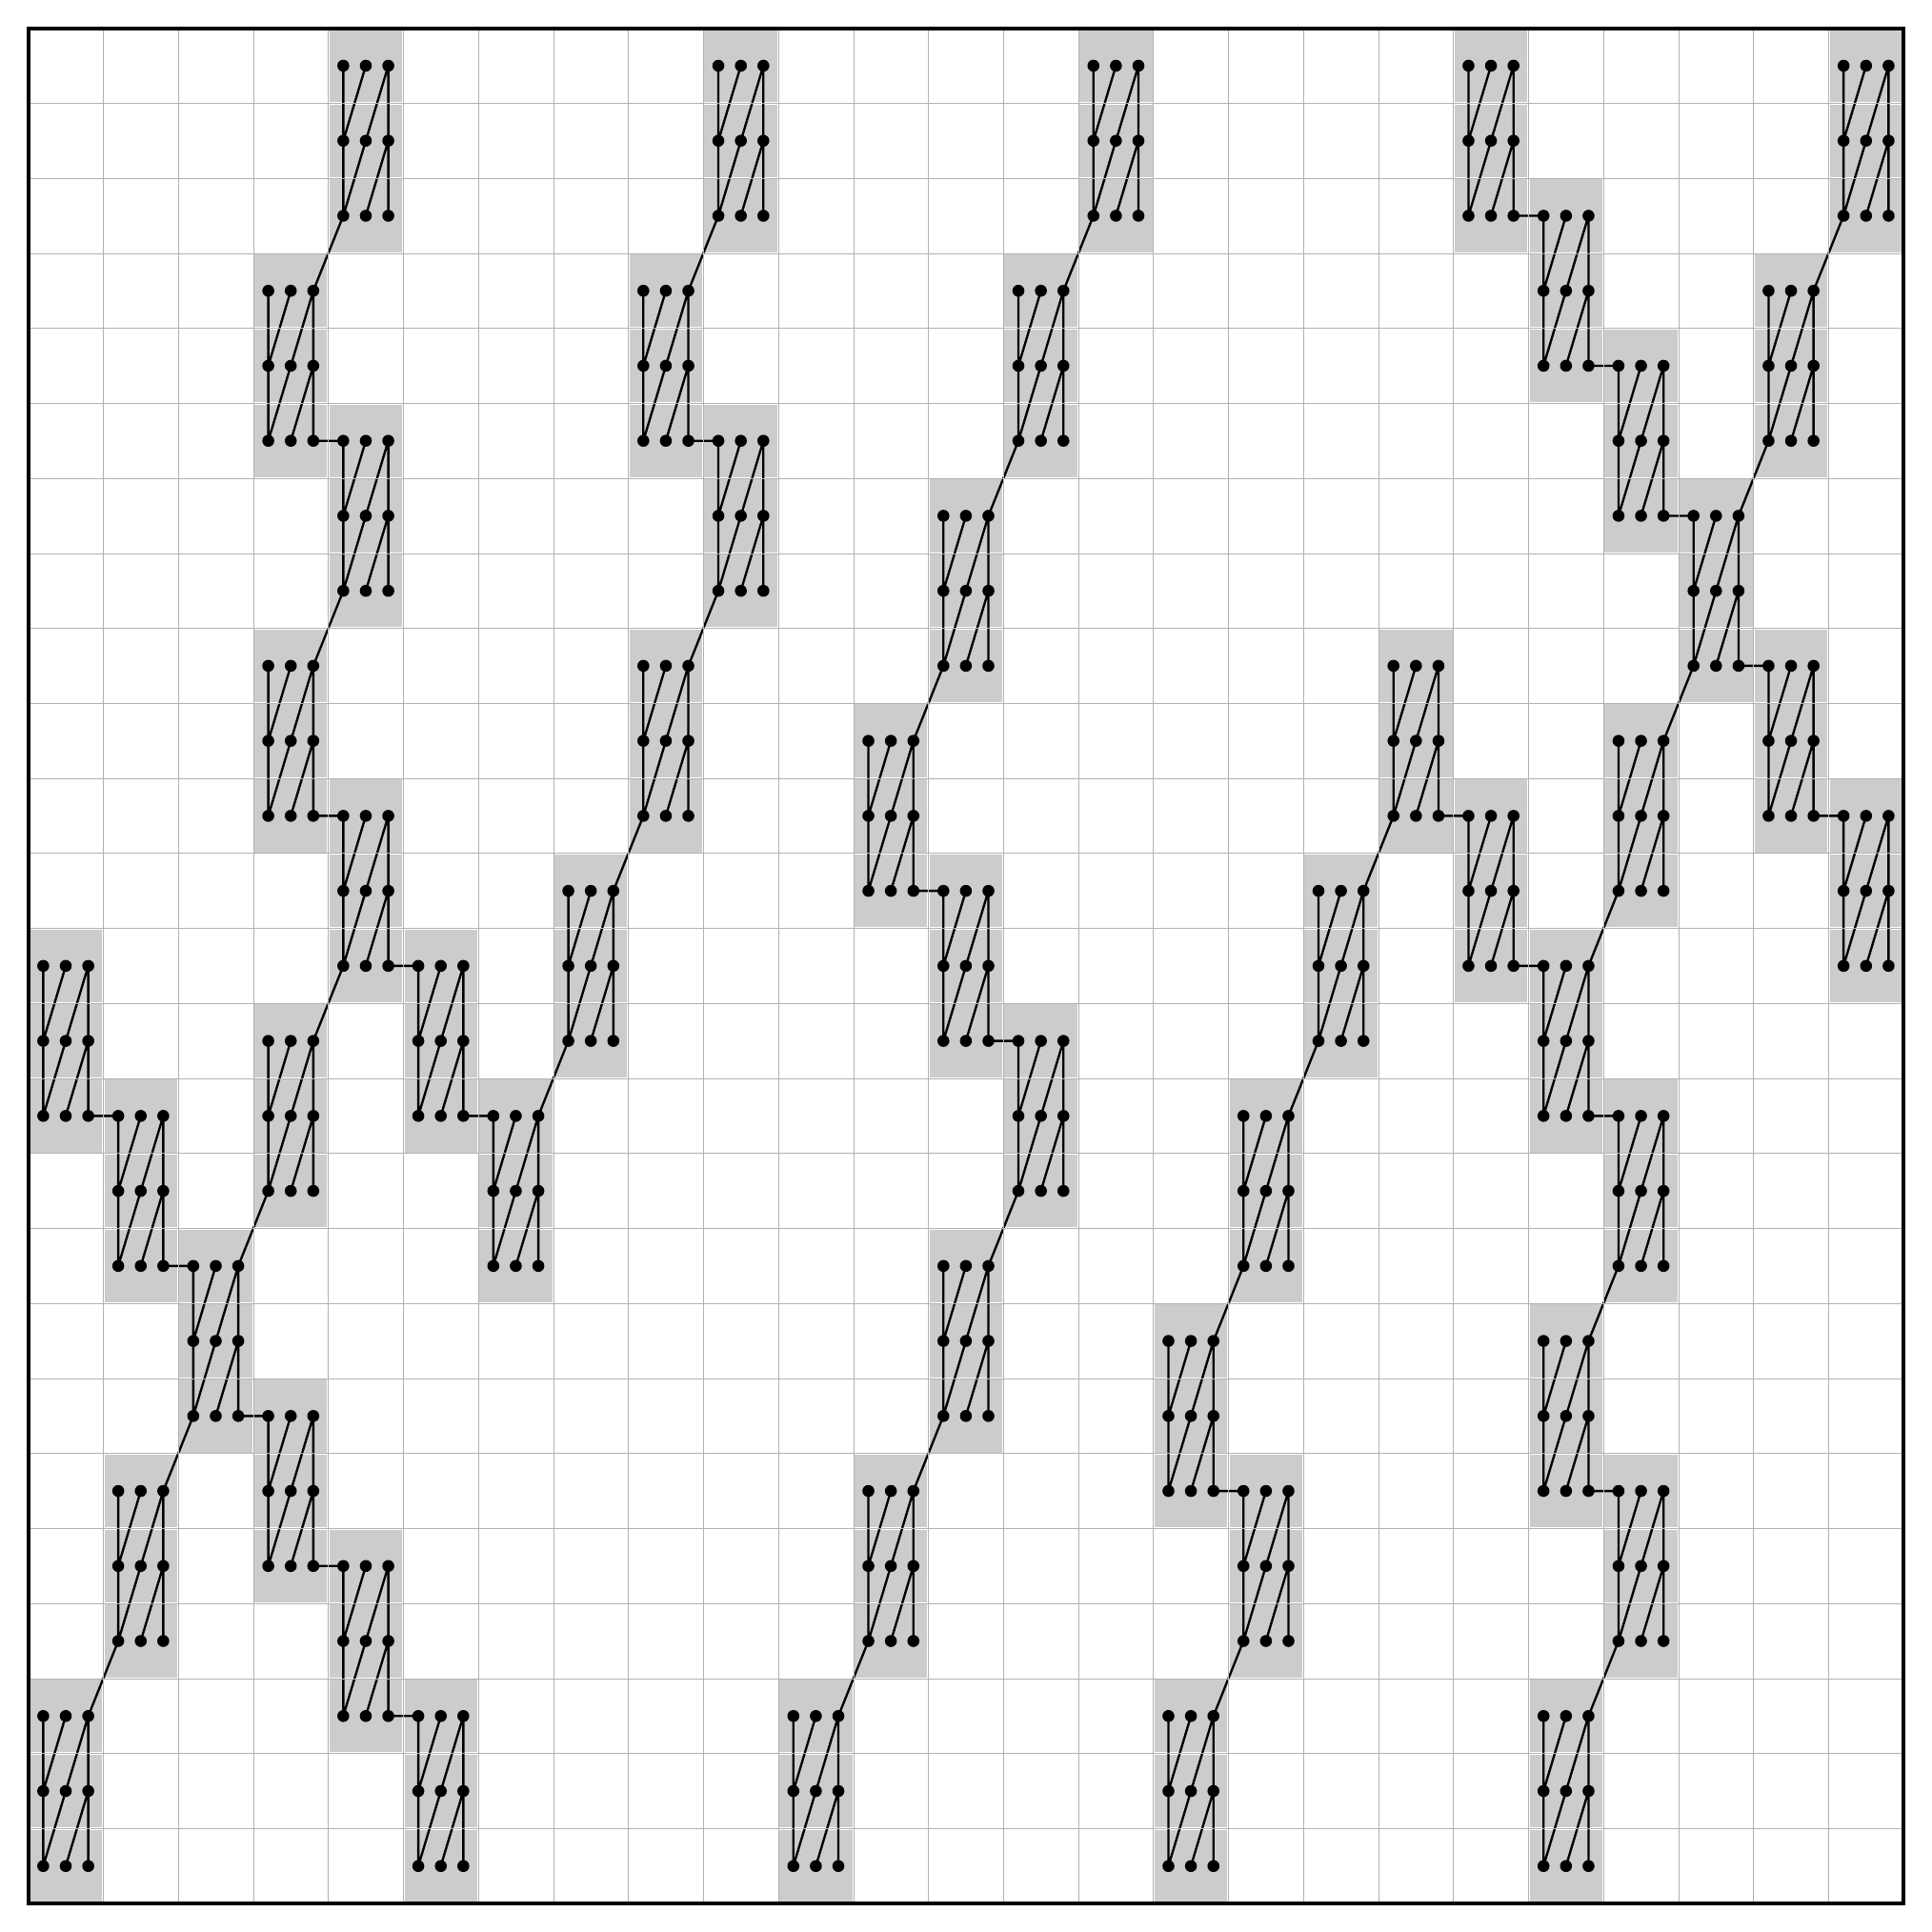
\begin{tikzpicture}
\foreach \a/\b in \D
    {
    \draw[black!0, fill=black!20, line width=0.3mm]
        (\a,\b) rectangle +(1,1)
        (\a,\b)++(0,1) rectangle +(1,1)
        (\a,\b)++(0,2) rectangle +(1,1);
    }
\foreach \a/\b in \D
    {
    \fill[black] foreach \c in 
        {(0.2, 0.5), (0.5, 0.5), (0.8, 0.5), (0.2, 1.5), (0.5, 1.5), (0.8, 1.5), (0.2, 2.5), (0.5, 2.5), (0.8, 2.5) }
        {(\a,\b)++\c circle (0.8mm)};
    \draw[black, line width=0.3mm]
        (\a,\b)++(0.2, 0.5)--+(0, 2)
        (\a,\b)++(0.2, 0.5)--+(0.6, 2)
        (\a,\b)++(0.8, 0.5)--+(0, 2)
        (\a,\b)++(0.2, 1.5)--+(0.3, 1)
        (\a,\b)++(0.5, 0.5)--+(0.3, 1);
    }
\draw[black, line width=0.3mm]
    foreach \a/\b in \A
        {(\a,\b)++(0.8, 2.5)--+(0.4, 1)}
    foreach \a/\b in \B
        {(\a,\b)++(0.2, 2.5)--+(-0.4, 0)};
\draw[help lines, black!30] (0,0) grid (25,25);
\draw[black, line width=0.5mm] (0,0)rectangle (25,25);
\end{tikzpicture}
\end{document}